\section{Multidimensional data organizations}

\subsection{Types of data and queries}

Let's consider multidimensional data representing points or regions in a k-dimensional space.

An example could be the following: consider a set of 8 records with two attributes A1 and A2 of type integer, which represent the latitude and longitude of cities, whose name will be used to denote the corresponding record, as shown in Picure \ref{multi_1}. Picture \ref{multi_2} provides a 2-dimensional representation of the points.

\begin{figure}[h!]
		\centering
		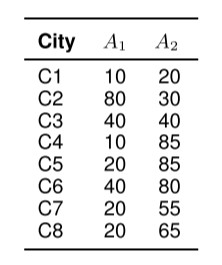
\includegraphics[scale = 1.5]{img/multi_1.jpg}
		\label{multi_1}
\end{figure}

\begin{figure}[h!]
		\centering
		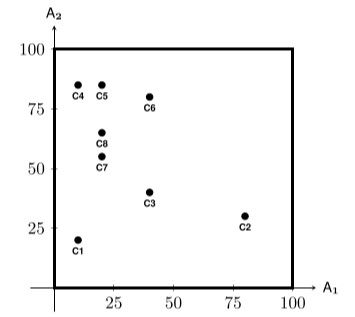
\includegraphics[scale = 1.5]{img/multi_2.jpg}
		\label{multi_2}
\end{figure}

The problems that will be considered are:

\begin{itemize}
    \item \textbf{primary organization}: how to divide stored data across pages;
    \item \textbf{secondary organization}: how to quickly find the region containing the points in a specified rectangular area. 
\end{itemize}

Both problems depend on the type of queries that are supported:

\begin{itemize}
    \item point/region search: check if a point/region is present;
    \item spatial range search: points/regions in a rectangle or ball;
    \item k-NN: find the k-closest points/regions with respect to a selected point/region.
\end{itemize}

\subsubsection{Multidimensional data organizations}
There exist different multidimensional data organizations.

\paragraph{Linear order based}
This organization let us to use traditional indexes in order to map positions, but it has a strong \textbf{precondition}: total order on the multidimensional data. Some examples of possible orders could be:

\begin{itemize}
    \item multi-attribute lexicographic order: in this case the points are store in a B+-tree. This order is useful for point search, but almost useless for range search and k-NN.

    \begin{figure}[h!]
		\centering
		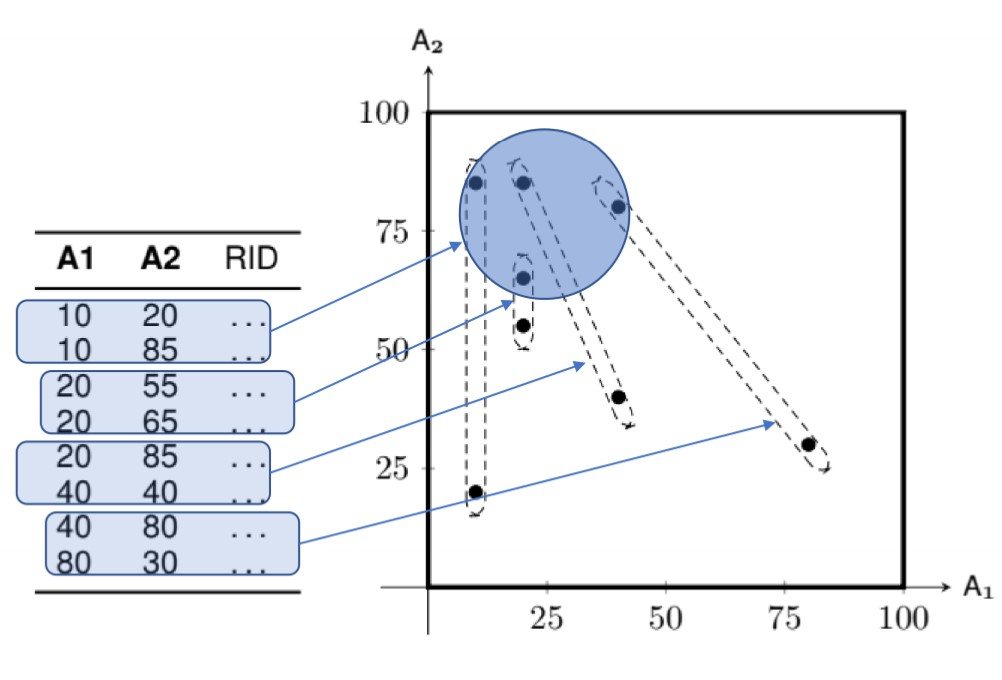
\includegraphics[scale = 0.8]{img/line1.jpg}
		\label{line1}
    \end{figure}

    \item diagonal order: in this case all the points are touched and it provides different type of granularity.

    \begin{figure}[H]
		\centering
		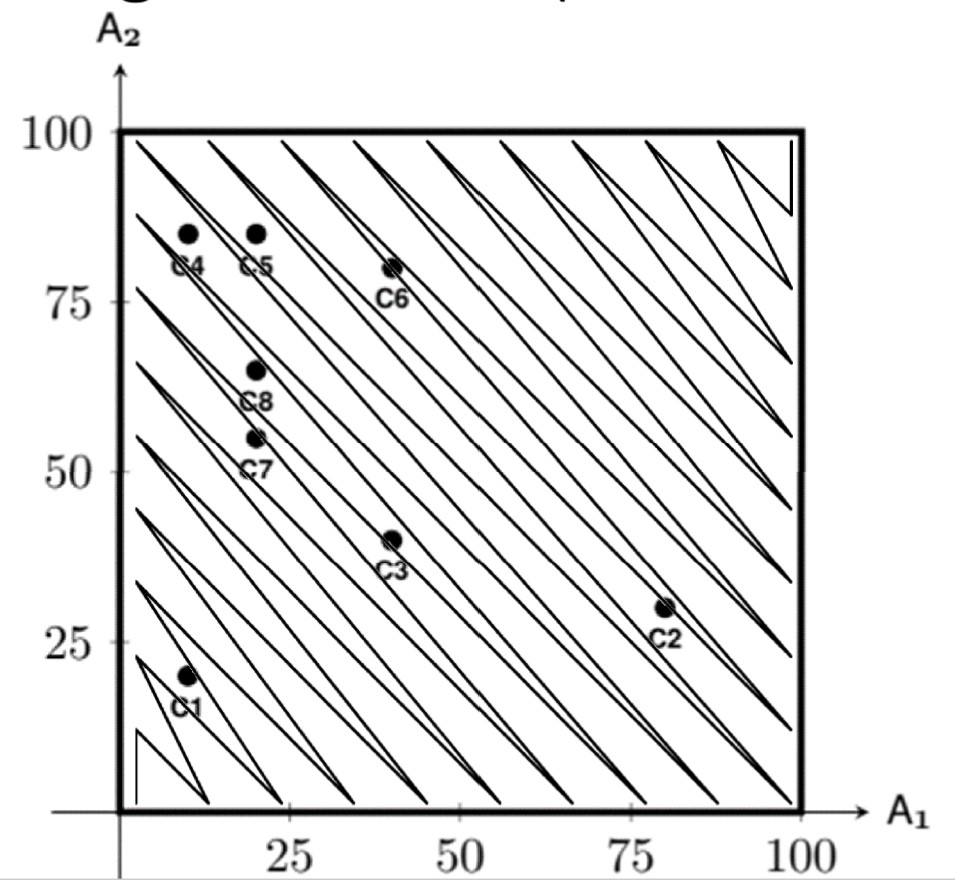
\includegraphics[scale = 0.7]{img/line2.jpg}
		\label{line2}
    \end{figure}

    \item Z-order

    \begin{figure}[h!]
		\centering
		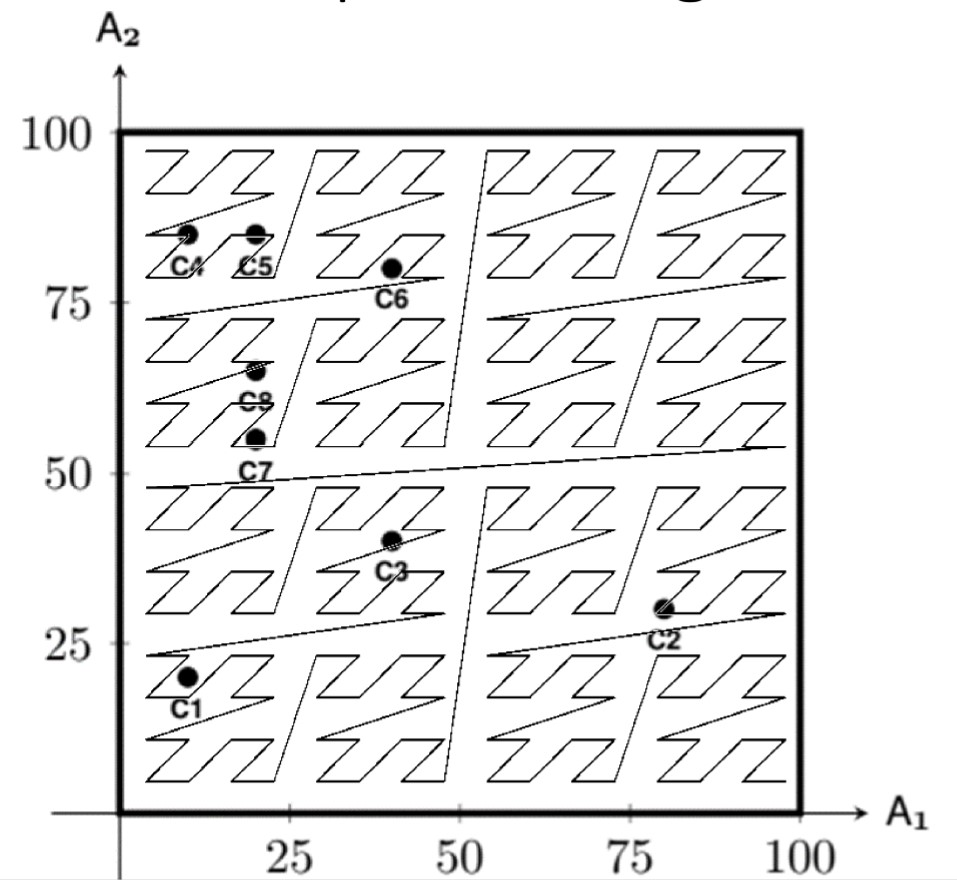
\includegraphics[scale = 0.7]{img/line3.jpg}
		\label{line3}
    \end{figure}

    \item Peano space filling curve

    \begin{figure}[h!]
		\centering
		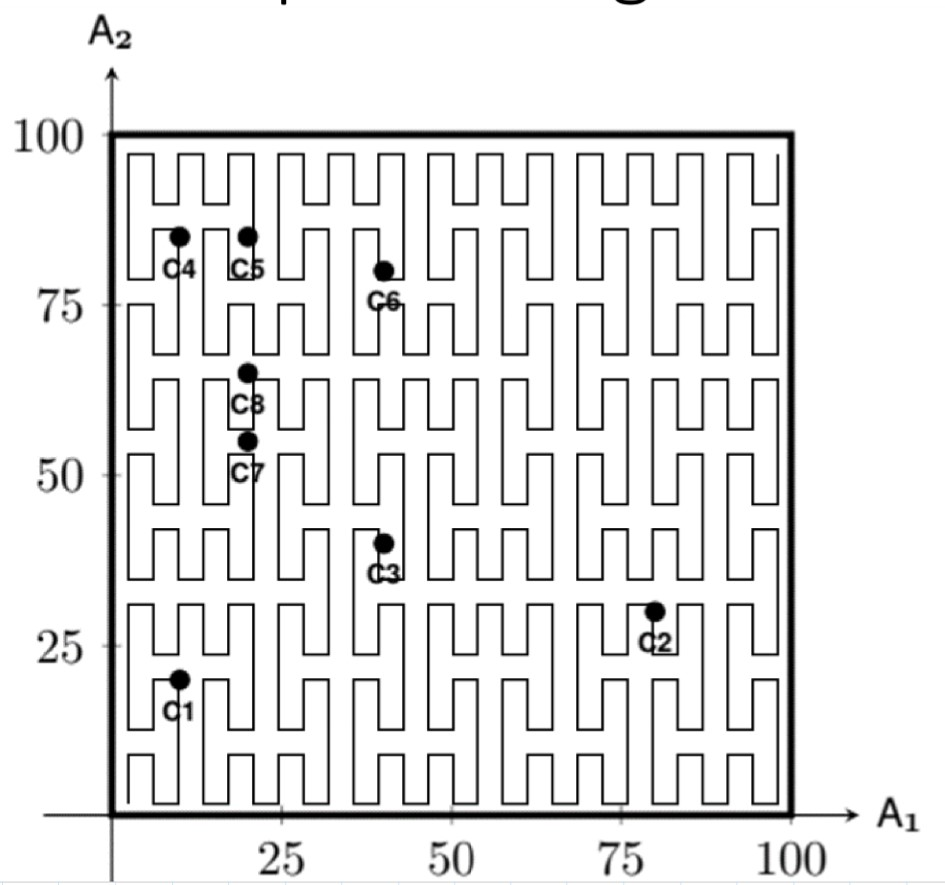
\includegraphics[scale = 0.7]{img/line5.jpg}
		\label{line5}
    \end{figure}

    \item Hilbert space filling curve

    \begin{figure}[H]
		\centering
		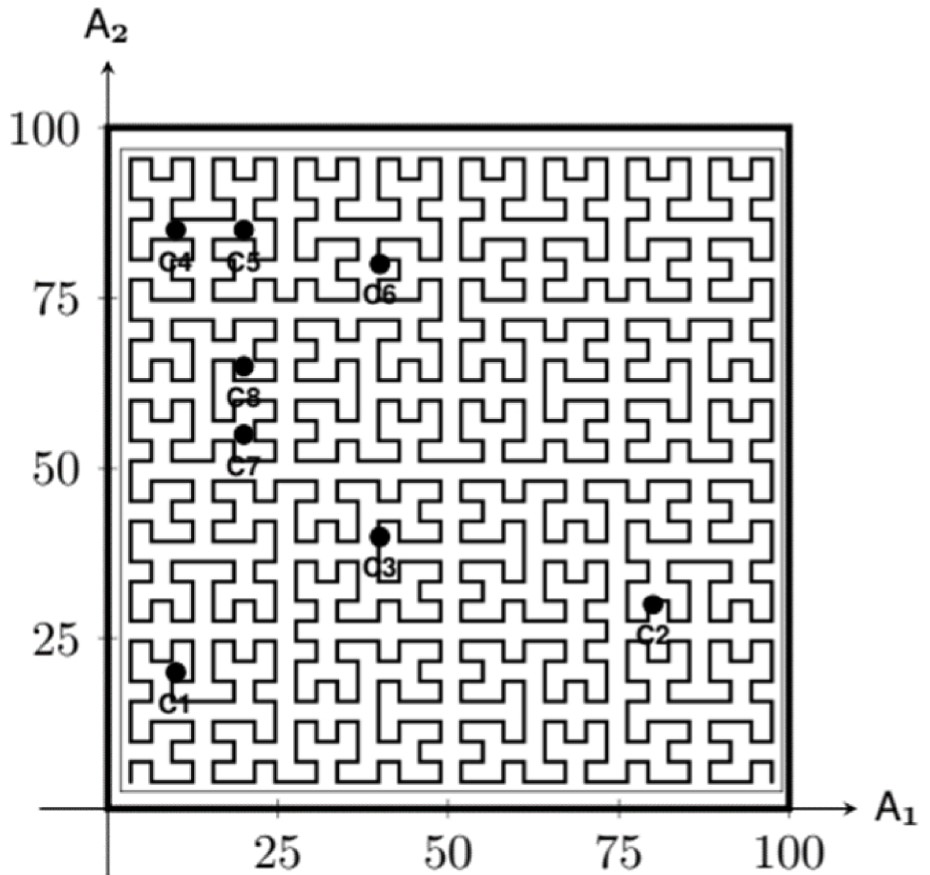
\includegraphics[scale = 0.7]{img/line4.jpg}
		\label{line4}
    \end{figure}
    
\end{itemize}

\subsubsection{Space partitioning}
In this case the focus is both on finding the partition of the space that results in (non-overlapping) regions that contain records that can be stored in a page and on how to quickly find the region containing the points for a specific query.

Let's focus on the different types of space partitioning:

\begin{itemize}
    \item classical partitioning: in this case the split is made according to a value of separation $d$ for a specific attribute. When there is a new overflow from a page during data loading, a new split is done, but changing the attribute.

    \begin{figure}[h!]
		\centering
		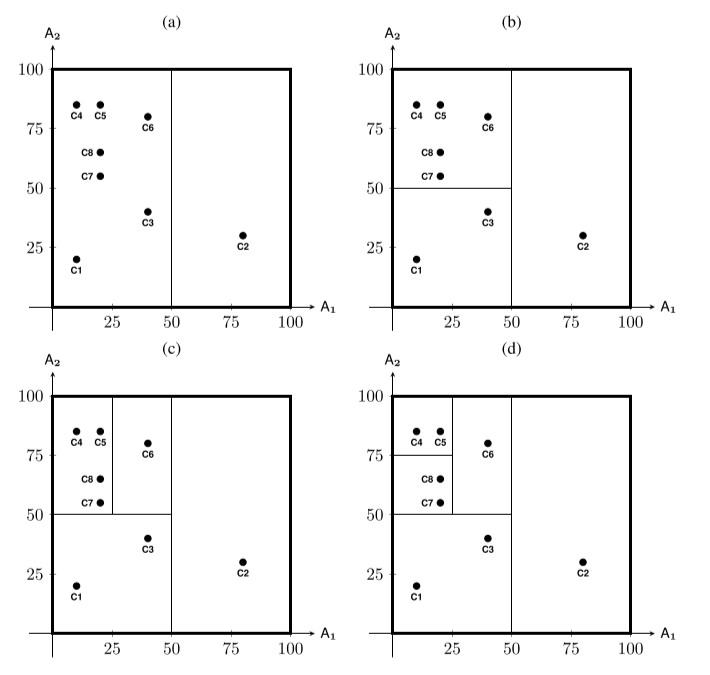
\includegraphics[scale = 1.2]{img/part1.jpg}
		\label{part1}
    \end{figure}

    \item point region quadtrees: this organization is used to organize bidimensional data, and it can be considered as the evolution of a binary tree into 2-dimension. Its limitation are:

    \begin{itemize}
        \item it is not balanced;
        \item it creates regions that are not needed;
        \item the higher the dimension, the higher the number of regions that are created.
    \end{itemize}

    \begin{figure}[h!]
		\centering
		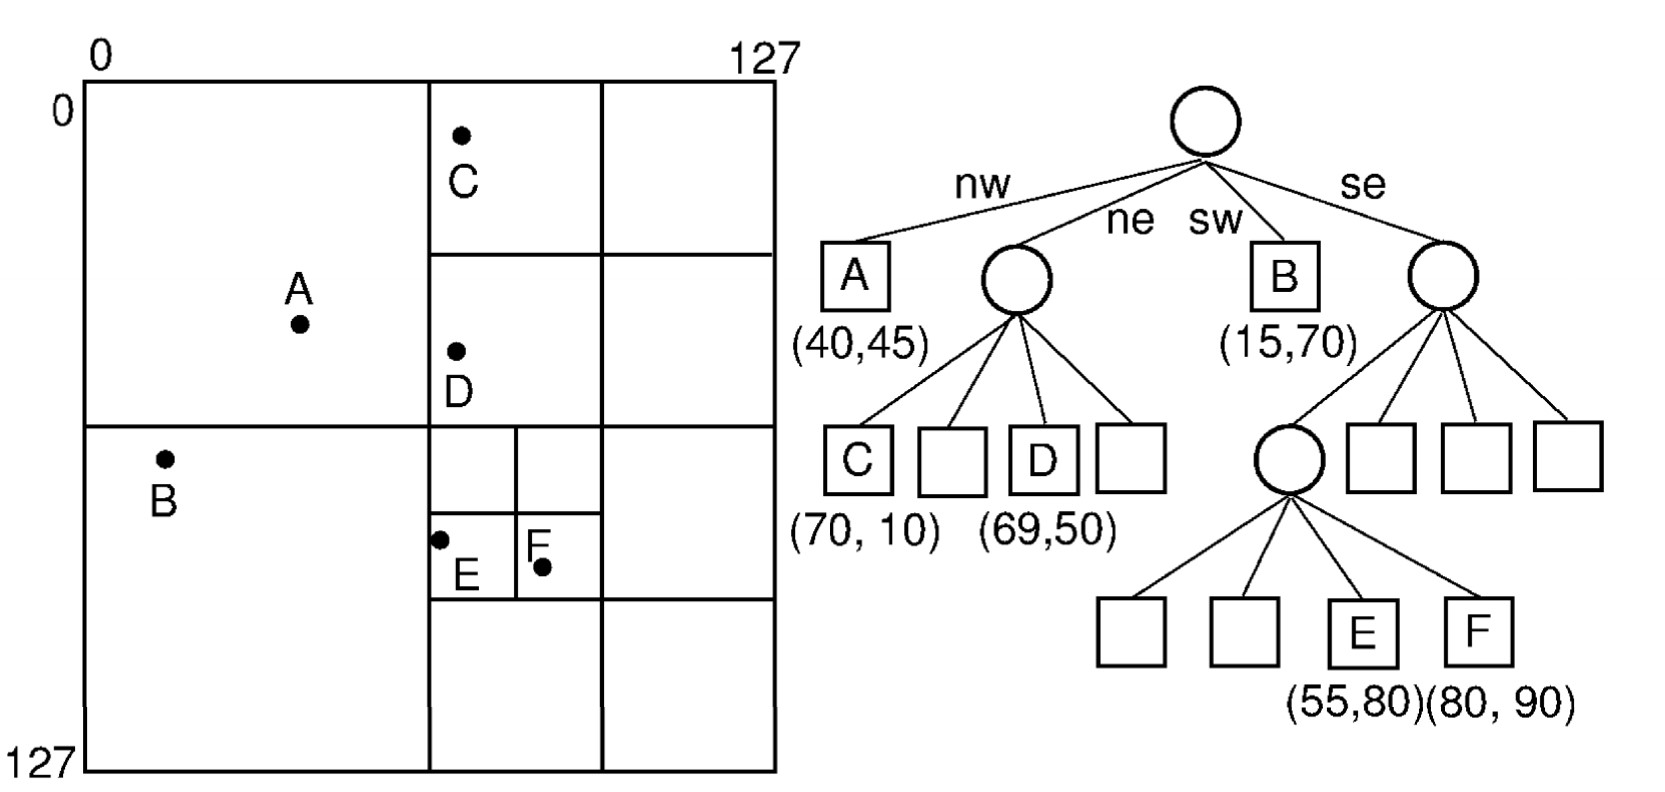
\includegraphics[scale = 0.5]{img/part2.jpg}
		\label{part2}
    \end{figure}

    
    \newpage
    \item octrees

    \begin{figure}[H]
		\centering
		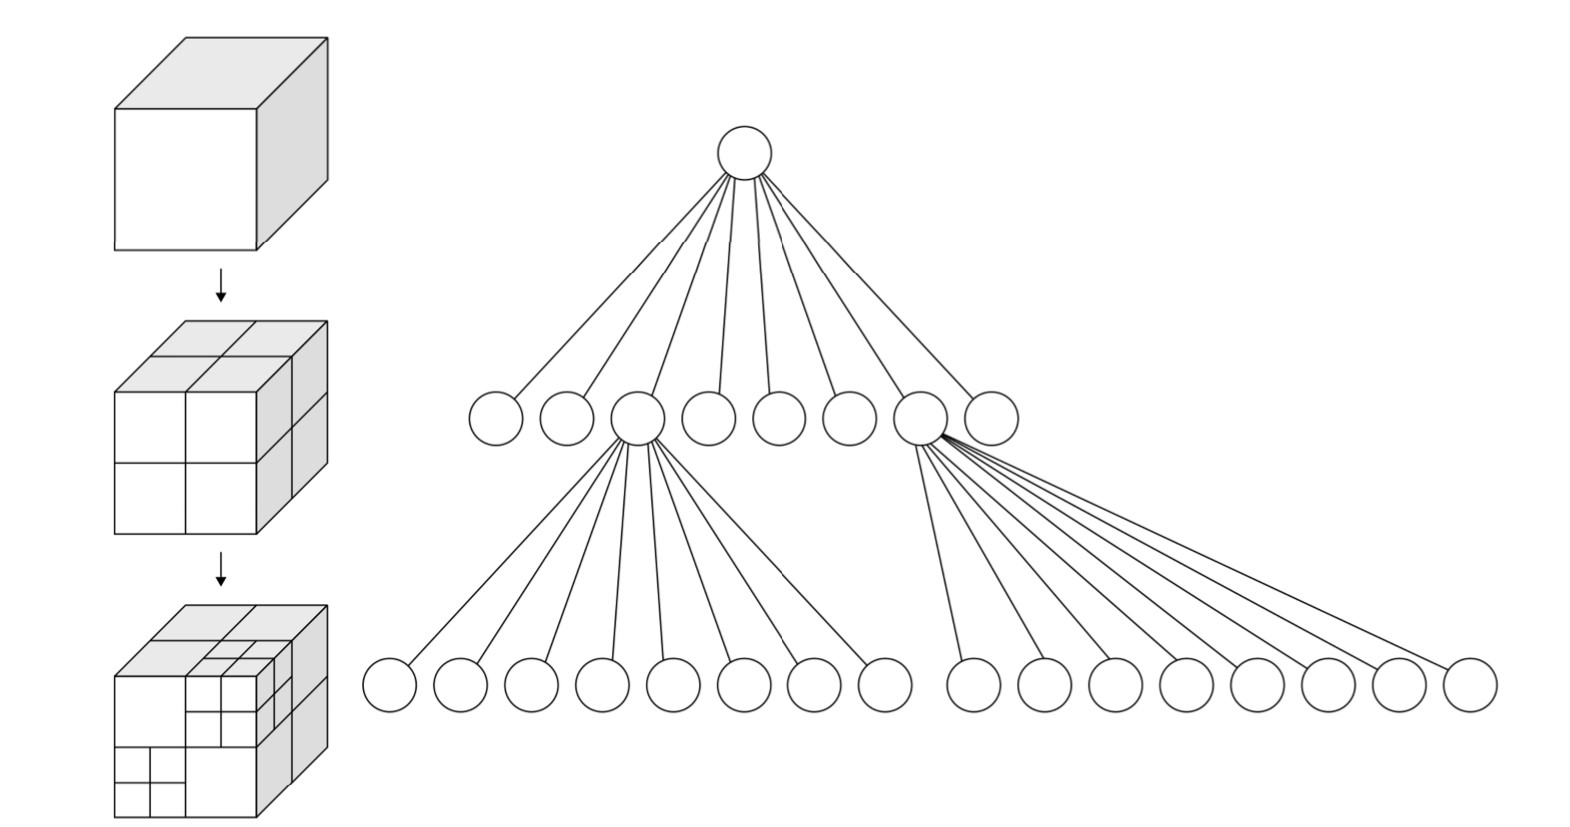
\includegraphics[scale = 0.5]{img/part3.jpg}
		\label{part3}
    \end{figure}

    \item KDB-trees: they inherit the idea of having a threshold to split the domain, but they use coordinates at time and they circle the order of the splitting strategy. In order to find the correct position, starting from the root is easier than starting from the leaves, because in this case an additional tree must be kept in order to manage the partition volume.

    \begin{figure}[h!]
		\centering
		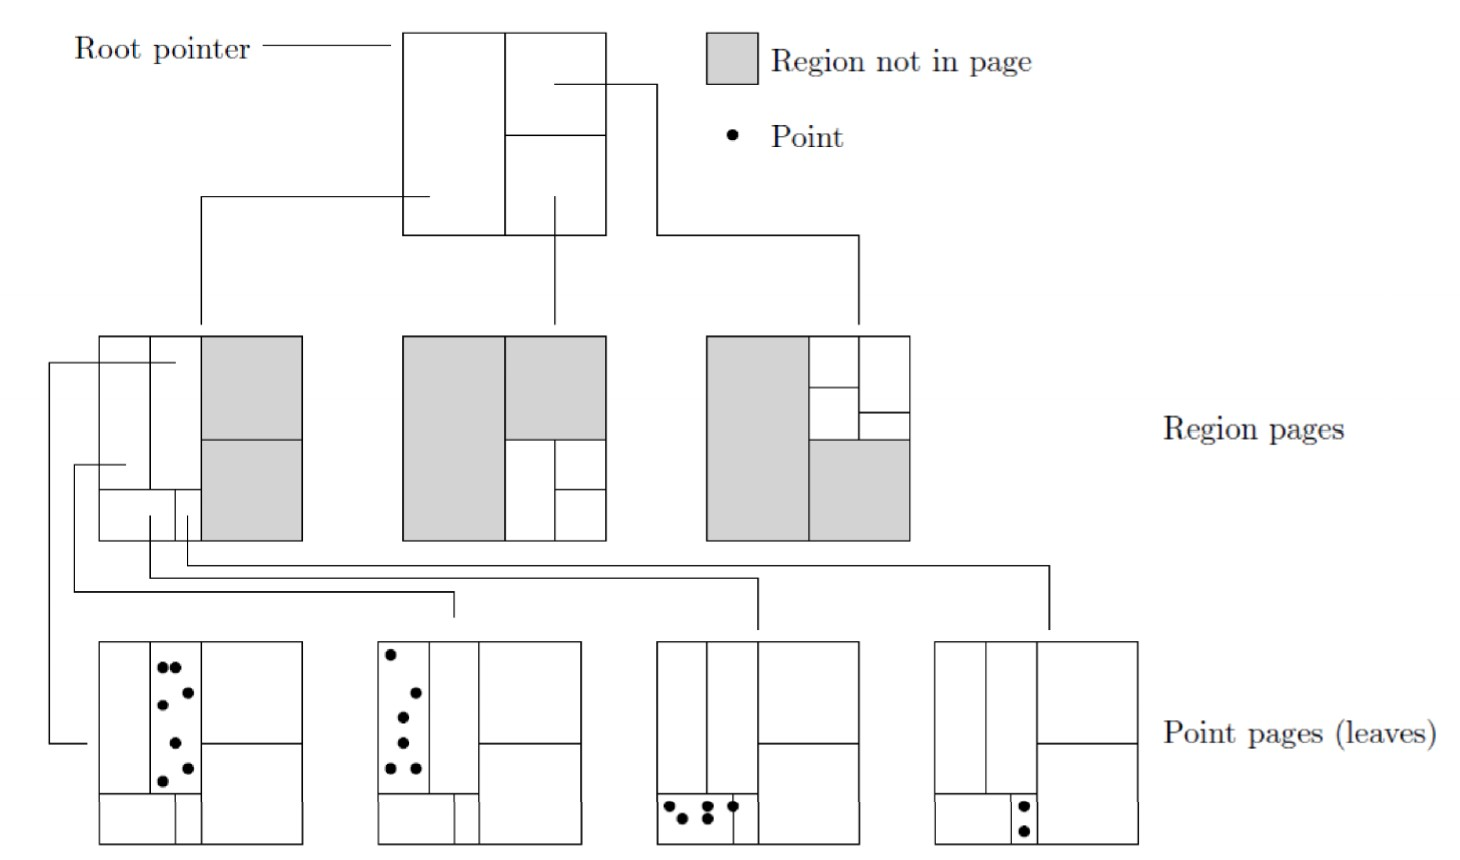
\includegraphics[scale = 0.7]{img/part4.jpg}
		\label{part4}
    \end{figure}
    
\end{itemize}

\subsubsection{G-trees}
\textbf{G-trees} combine the ideas of data partitioning and of B+-trees as follows: data space is divided into non-overlapping regions of variable size identified by an appropriate code, then a total ordering is defined for partition codes, and they're stored in a B+-tree. If we consider a 2-dimensional case, assuming that data pages may contain 2 points, then a \textbf{partition code} is a binary string constructed as follows:

\begin{itemize}
    \item the initial region is identified by the empty string;
    \item the first split is made along the X-axis, and the two partitions it produces are "0" and "1". Points $0 < x \leq 50$ are in partition "0", while points $50 < x \leq 100$ belong to partition "1";
    \item when a partition of the previous step is split along Y-axis, then the new partition codes become "00" and "01" and so on...
\end{itemize}

An example of G-tree is showed in Picture \ref{part5}.

\begin{figure}[H]
		\centering
		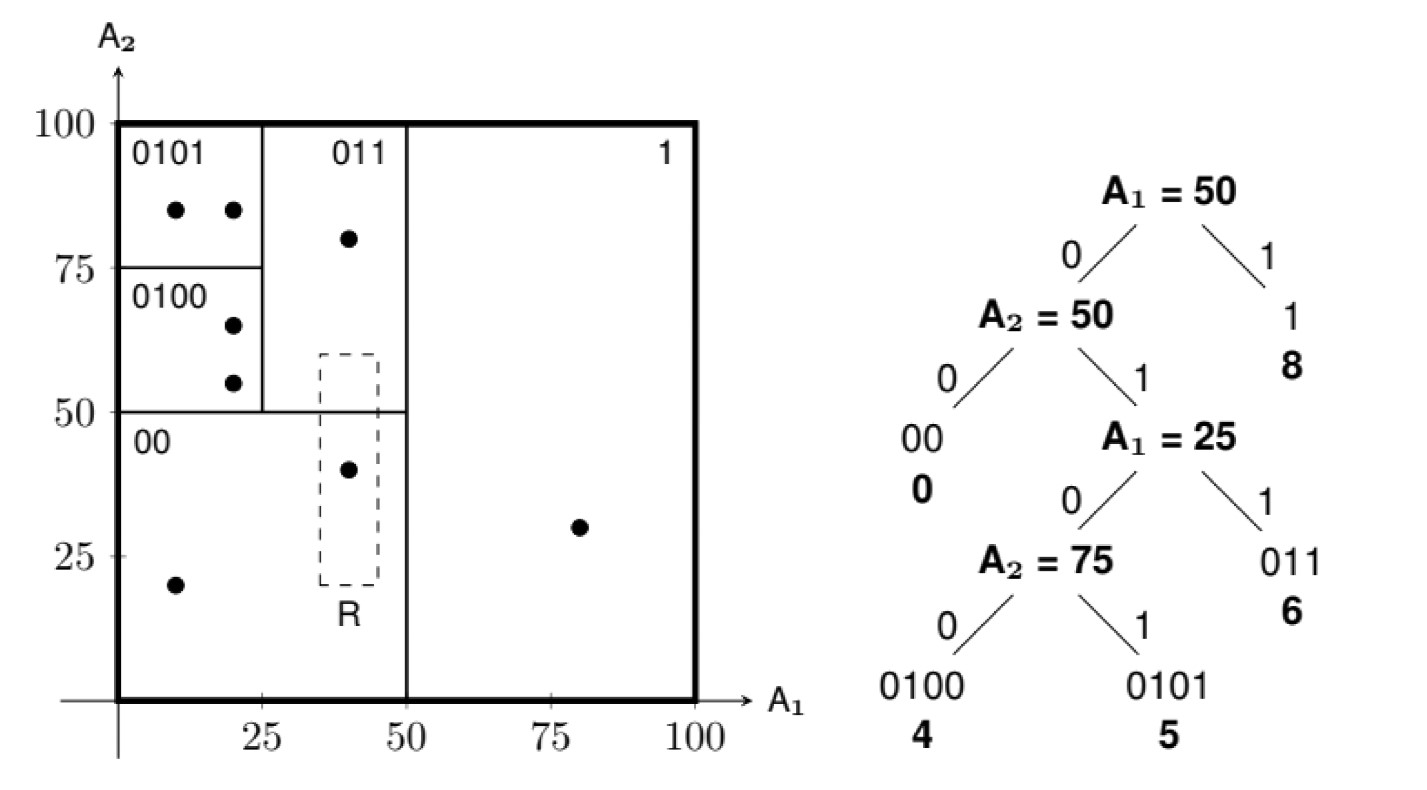
\includegraphics[scale = 0.7]{img/part5.jpg}
        \caption{Example of G-tree}
		\label{part5}
\end{figure}

The Picture \ref{part6} represents the partition codes and the B+-tree which is used to store them.

\begin{figure}[H]
		\centering
		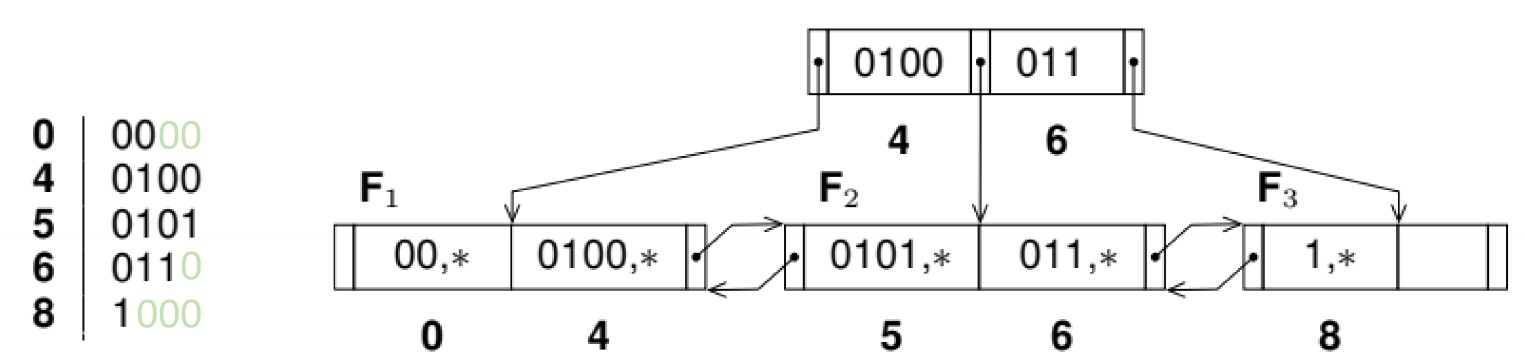
\includegraphics[scale = 0.7]{img/part6.jpg}
        \caption{Example of G-tree}
		\label{part6}
\end{figure}

\paragraph{Operations}

Now we focus on some possible operations which can be performed using these G-trees:

\begin{itemize}
    \item \textbf{point search}: let $M$ be the maximum length of the partition number of the G-tree, then the search for a point $P$ with coordinates $(x,y)$ proceeds as follows:

    \begin{enumerate}
        \item the partition tree is searched for the code $S_p$ of the partition that contains $P$, if it is present
        \item the G–tree is searched for the partition code $S_p$ to check if $P$ is in the associated page.
    \end{enumerate}
    
    \item \textbf{spatial range search}: a spatial range search looks for the points $P_i$ with coordinates $(x_i, y_i)$ such that $x_1 \leq x_i \leq x_2$ and $y_1 \leq y_i \leq y_2$, i.e. they are in the query region $R = \{ (x_1, y_1), (x_2, y_2) \}$. The query result is found as follows:

    \begin{enumerate}
        \item the G–tree is searched for the leaf node $F_h$ of the partition containing the lower left vertex $(x_1, y_1)$ of $R$
        \item the G–tree is searched for the leaf node $F_k$ of the partition containing the upper right vertex $(x_2, y_2)$ of $R$
        \item for each leaf from $F_h$ to $F_k$ the elements S are searched such that $R_S = RegionOf(S)$ overlaps with the query region $R$, where $RegionsOf(S)$ is a function that maps the code $S$ of a partition R in the coordinates of the lower left and upper right vertices of the partition
    \end{enumerate}

    \item \textbf{point insertion}: 

    \begin{enumerate}
        \item the G–tree is searched for the leaf node $F$ of the partition $R_p$ that should contain it. Let $S_p$ be the code of $R_p$
        \item if $R_p$ is not full, insert $P$, otherwise $R_p$ is split in $R_p_1$ and $S_p_1$, with codes $S_p_1 = S_p$“0” and $S_p_2 = S_p$“1”. If the new strings have a length greater than $M$, $M$ takes the value $M+1$
        \item the points in $R_p$ and $P$ are distributed in $RP1$ and $R_P_2$. 
        \item the element ($S_p$, $p_R_p$) in the leaf $F$ is replaced by ($S_p_1$, $p_R_p_1$) and ($S_p_2$, $p_R_p_2$)
    \end{enumerate}

    \item \textbf{point deletion}:
    \begin{enumerate}
        \item let $F$ be the leaf node with the partition $R_p$ containing $P$, $S_p$ the partition code of $R_p$, and $S$' the partition code of $R$' obtained from $R_p$ with a split and therefore different from $S_p$ for the last bit only
        \item $P$ is deleted from $R_p$ and then two cases are considered:
        \begin{itemize}
            \item $R$' has been split:
            \begin{itemize}
                \item If the partition $R_p$ becomes empty, then $S_p$ is deleted
                \item Otherwise the operation terminates
            \end{itemize}
            \item $R$' has not been split:
            \begin{itemize}
                \item If the two partition cannot be merged, the operation terminates
                \item Otherwise the two partition are merged
            \end{itemize}
        \end{itemize} 
    \end{enumerate}
\end{itemize}

\subsubsection{R*-trees}
\begin{itemize}
    \item an R*-tree is a dynamic tree structure perfectly balanced as a B+-tree, used for retrieval of multidimensional data according to ita spatial position;
    \item terminal nodes of a R*-tree contain elements of the form $(R_i, O_i)$, where:
    \begin{itemize}
        \item $R_i$ is the rectangular data;
        \item $O_i$ is its reference to the data nodes; for simplicity we denote $O_i$ as *.
    \end{itemize}  
    \item non terminal nodes contain elements of type $(R_i, p_i)$, where 
    \begin{itemize}
        \item $p_i$ is a reference to the root of a subtree;
        \item $R_i$ is the minimum bounding rectangle countaining all rectangles associated with the child nodes.
    \end{itemize}
\end{itemize}

\begin{figure}[H]
		\centering
		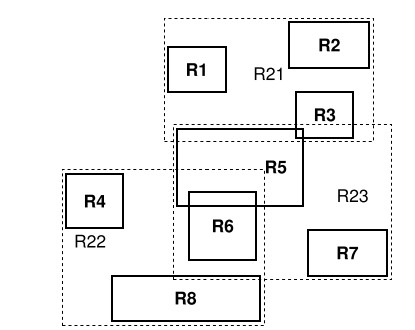
\includegraphics[scale = 1.3]{img/part7.jpg}
		\label{part6}
\end{figure}

\begin{figure}[H]
		\centering
		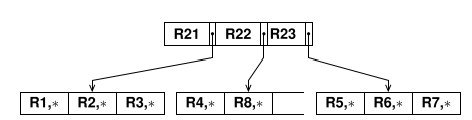
\includegraphics[scale = 1.5]{img/part8.jpg}
		\label{part6}
\end{figure}

The \textbf{properties} of R*-tree are:
\begin{itemize}
    \item each node has a number of elements between $m = $ the minimum number of elements in a node, and $M = $ the maximum;
    \item all leaf nodes are at the same level;
\end{itemize}

\textbf{Differences} with B+-trees:
\begin{itemize}
    \item there is no sort order in R*-trees, unlike B+-trees;
    \item there may be overlap between regions associated with different elements of the same level, unlike B+-trees.
\end{itemize}

\paragraph{Operations}

\begin{itemize}
    \item \textbf{search overlapping data regions}: suppose we want to search all the overlapping regions to the region $R$:
    \begin{itemize}
        \item the root is visited in order to look for elements $(R_i, p_i)$, with $R_i$ that overlaps with $R$;
        \item for each element $(R_i, p_i)$ found, the search proceeds in the subtree rooted in $p_i$: when a leaf node is reached, the data regions $R_i$ in the search results are those with $R_i$ that overlaps with $R$.
    \end{itemize}
    
    \begin{figure}[H]
		\centering
		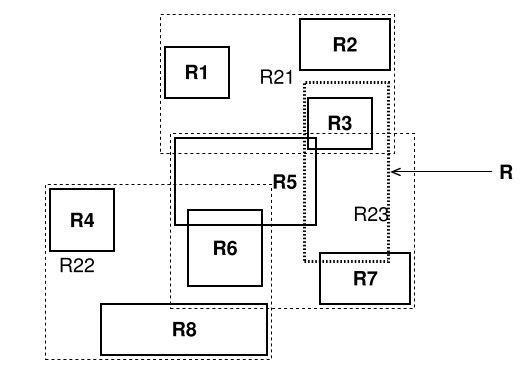
\includegraphics[scale = 1.5]{img/part9.jpg}
		\label{part6}
    \end{figure}
    
    In the example, $R_3, R_5$ and $R_7$ overlaps with $R$.

    \item \textbf{insertion}: let $S$ be a new data region to insert. The operation is similar to inserting a key in a B+-tree, since $S$ is stored in a leaf node, and if there is an overflow, the node will be split into two nodes. In the worst case the division can propagate to the parent node up to the root. However, there is a significant difference with the insertion in B+-trees: in R*-trees, since the regions may overlap, the new data region $S$ may overlaps with more of them, so it could be inserted in more leaf nodes. In this sense, the choice of the region in an internal node can be made according to the degree of overlap with $S$. After having selected the node $N$ where to insert $S$, if an overflow does not occur, the region is recalculated and its value propagates in the parent node, otherwise:

    \begin{enumerate}
        \item if it is the first overflow, then a fraction $p$ of the $M+1$ entries are removed from the node and reinserted in the tree, in a sort of dynamic reorganization of the tree
        \item otherwise, the $M+1$ elements are divided between two nodes, and two new elements are inserted in the parent node, and the process goes on to propagate the effects.
    \end{enumerate}

    \underline{Example}: assume to insert region $S$ (a): the process starts with the root node of the R*-tree in (c). Let the region $R21$ be selected for the insertion. Following the associated pointer, the leaf node to the left is considered, and since this node does not have enough space to contain $S$ an overflow occurs. Being the first, we proceed with the reinsertion of R1. The region $R21$ is updated (not shown in the figure) and the reinsertion takes place in the same leaf node, causing another overflow and then a subdivision. Suppose that we get ${R1, S}$ and ${R2, R3}$. Let $R24$ and $R25$ be the regions containing $(R1, S)$ and $(R2, R3)$ (b). Consequently, two new elements have to be inserted into the root node to replace $R21$ (c). Since in the root node there is not enough space to contain four elements, there is an overflow. In the root the reinsertion it is not applied, but a subdivision is made. The result is that the old root node is replaced by two new nodes, one containing $(R24, R25)$ and the other $(R22, R23)$. Let $R26$ be the region containing $(R24, R25)$ and $R27$ be the region containing $(R22, R23)$. A new root is added with elements $R26$ and $R27$ (d).

    \begin{figure}[h!]
		\centering
		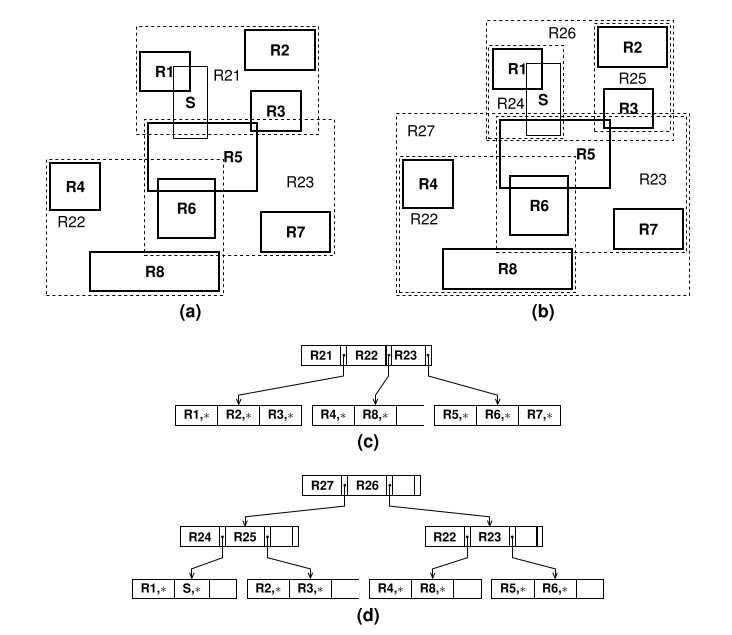
\includegraphics[scale = 1.6]{img/part10.jpg}
		\label{part6}
    \end{figure}
\end{itemize}